%%%%%%%%%%%%%%%%%%%%%%%%%%%%%%%%%%%%%%%%%
% Imperial College London Presentation
% LaTeX Template
% Version 1.0 (April 16, 2024)
%
% This template was created by:
% Vel (enquiries@latextypesetting.com)
% LaTeXTypesetting.com
%
%!TEX program = xelatex
% Note: this template must be compiled with XeLaTeX rather than PDFLaTeX
% due to the custom fonts used. The line above should ensure this happens
% automatically, but if it doesn't, your LaTeX editor should have a simple toggle
% to switch to using XeLaTeX.
%
% © Imperial College London, 2024. This template, including logo and fonts, is 
% for use of Imperial staff and students only for university business. All rights 
% reserved to the copyright owners.
%
%%%%%%%%%%%%%%%%%%%%%%%%%%%%%%%%%%%%%%%%%

%----------------------------------------------------------------------------------------
%	CLASS, PACKAGES AND OTHER DOCUMENT CONFIGURATIONS
%----------------------------------------------------------------------------------------

\documentclass[
aspectratio=169, % Uncomment to use an aspect ratio of 16:9 (160 mm by 90 mm)
%aspectratio=43, % Uncomment to use an aspect ratio of 4:3 (128mm by 96mm)
t, % Top align all slide content by default
onlytextwidth, % Typeset content in columns at text width
10pt, % Default font size, use 10pt for the 16:9 aspect ratio and 8pt for the 4:3 aspect ratio
]{beamer}

\usetheme{Imperial} % Use the Imperial theme

%----------------------------------------------------------------------------------------
%	IMPERIAL BEAMER THEME USAGE NOTES
%----------------------------------------------------------------------------------------

% This theme features several predefined Imperial colors which can be used for text and slide backgrounds:
% ICLBlue - Most common slide background color and text color to use (on light backgrounds)
% ICLDarkBlue - Optional darker blue color for slide backgrounds and text
% ICLCream - Accessible background color for use on slide backgrounds
% ICLLightGrey - Accessible background color for use on slide backgrounds

% You can choose to use a 16:9 aspect ratio (default) or a 4:3 aspect ratio by uncommenting the relevant line in the \documentclass specifications above. Note that if you switch between the 2 aspect ratios, you will likely need to adjust how your images are included in the presentation. Usually for a 16:9 aspect ratio, images will be included as width=\paperwidth, but for a 4:3 aspect ratio it's recommended to use height=\paperheight instead.

%----------------------------------------------------------------------------------------
%	PRESENTATION INFORMATION
%----------------------------------------------------------------------------------------

\title{A Crash Course on Lattices} % Presentation title to appear on the title slide and left footers

\subtitle{and how they're building the future of cryptography} % Presentation subtitle to appear on the title slide

\author{Joshua Limbrey} % Author name(s) to appear on the title slide

\date{2024-03-22} % Presentation date to appear on the title slide and right footers


%----------------------------------------------------------------------------------------
%   SET MATHS FONT AND ITALICS
%----------------------------------------------------------------------------------------
\usefonttheme[onlymath]{serif}
\usepackage{newtxtext, newtxmath}
\usepackage{soul} % for strikethrough
\usepackage{multicol}
\usepackage{algorithm}
\usepackage{algpseudocode}
\usepackage{wrapfig}
\usepackage[style=alphabetic,]{biblatex}
\usepackage{amsthm}
\usepackage{tcolorbox}
\usepackage[dvipsnames]{xcolor}

\addbibresource{bib.bib}

%----------------------------------------------------------------------------------------

\begin{document}

%----------------------------------------------------------------------------------------
%	TITLE SLIDES
%----------------------------------------------------------------------------------------

% Select one of the 3 title slide types below and remove or comment out the others

%------------------------------------------------

% Blue background title slide example

\begingroup
\setbeamercolor{background canvas}{bg=ICLBlue} % Slide background color
\setbeamercolor{title page title}{fg=white} % Title text color
\setbeamercolor{title page subtitle}{fg=white} % Subtitle text color
\setbeamercolor{author}{fg=white} % Author(s) text color
\setbeamercolor{date}{fg=white} % Date text color
\setbeamertemplate{title page}[logo]{ICL_Logo_White.pdf} % Imperial logo color, use 'ICL_Logo_White.pdf' for white and 'ICL_Logo_Blue.pdf' for blue
\frame[plain, s]{\titlepage} % Output the title page with no footer ('plain') and vertically distributed text ('s')
\endgroup

%----------------------------------------------------------------------------------------
%	AGENDA SLIDES
%----------------------------------------------------------------------------------------

% White agenda slide

\begingroup
\setbeamercolor{normal text}{fg=ICLBlue}\usebeamercolor[fg]{normal text} % Slide text color

\begin{frame}
    \begin{columns}[T] % [T] ensures correct vertical alignment
        \begin{column}{0.48\linewidth} % Left column
            \HUGE\textbf{Agenda}
        \end{column}
        \begin{column}{0.48\linewidth} % Right column
            \textbf{01}\tabto{0.125\linewidth} What is currently used for cryptography?\\ % Use \tabto{<length>} to add a fixed horizontal whitespace
            \textbf{02}\tabto{0.125\linewidth} What is a lattice?\\
            \textbf{03}\tabto{0.125\linewidth} What are these ``hard lattice problems''?\\
            \textbf{   }\tabto{0.25\linewidth} Closest Vector Problem\\
            \textbf{   }\tabto{0.25\linewidth} Learning with Errors\\
            \textbf{   }\tabto{0.25\linewidth} Lattice Isomorphism Problem\\
            \textbf{04}\tabto{0.125\linewidth} The PQC Timeline\\
            \textbf{05}\tabto{0.125\linewidth} Further reading
        \end{column}
    \end{columns}
\end{frame}
\endgroup

%----------------------------------------------------------------------------------------
%	PRESENTATION BODY SLIDE EXAMPLES
%----------------------------------------------------------------------------------------

\begin{frame}
    \frametitle{What is currently used for cryptography?}

    \begin{columns}[T] % [T] ensures correct vertical alignment
        \begin{column}{0.33\linewidth} % Left column
            \begin{itemize}
                \item Diffie-Hellman
                \item El Gamal
                \item RSA
                \item DSA
                \item ECDSA
                \item ECDH
                \item Ed25519
            \end{itemize}
        \end{column}
        \begin{column}{0.63\linewidth} % Right column
            All public key cryptography relies on what is called a \textbf{trap-door function}.

            Easy to go one way \textit{(encrypt)}, difficult to go the other \textit{(decrypt)} without knowledge of a secret \textit{(private key)}.

            All of the schemes listed to the left are all dependant on the hardness of \textbf{prime factorisation} or the \textbf{discrete logarithm problem}.
        \end{column}
    \end{columns}
\end{frame}

%------------------------------------------------

\begin{frame}
    \frametitle{Why are we bored of these?}
    \begin{columns}[T] % [T] ensures correct vertical alignment
        \begin{column}{0.48\linewidth} % Left column
            These schemes have been around for a while (some nearly 50 years). The security against a standard adversary has been extensively studied, and the hardness of the problems fairly well understood.

            Challenging to construct new and interesting forms of encryption (such as \textit{homomorphic encryption}) due to the properties of the underlying problems.

            Shor's algorithm\footfullcite{shor} means that given an adversary with a sufficiently strong quantum computer, these schemes are no longer secure.
        \end{column}
        \begin{column}{0.48\linewidth} % Right column
            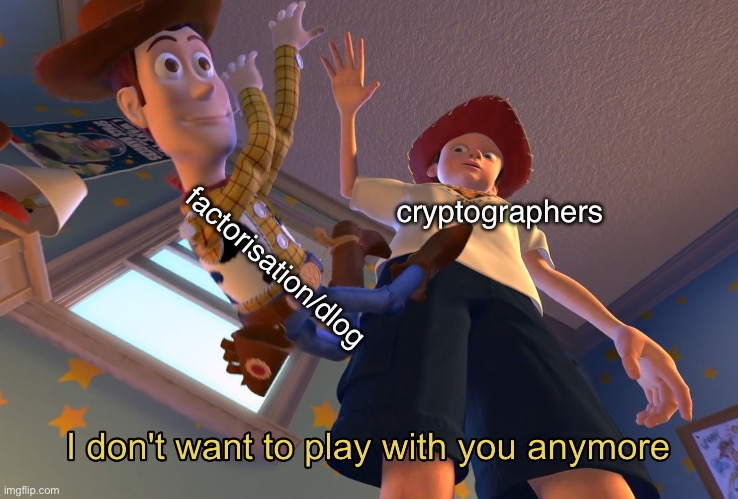
\includegraphics[width=\linewidth]{toy_story.jpeg} % Trimming is used to crop your image and the order of dimensions is: left, bottom, right, top. It's recommended to crop outside of LaTeX though, to ensure the aspect ratio remains the same.
            {\tiny\textcolor{ICLBlue}{(Above) Cryptographers wanting new toys, circa 2000 (colourised)}}
        \end{column}
    \end{columns}
\end{frame}

%------------------------------------------------

\begin{frame}
    \frametitle{What is a lattice?}
    \begin{columns}[T]
        \begin{column}{0.48\linewidth}
            \begin{center}
            \begin{tcolorbox}[colback=ICLBlue!5!white,colframe=ICLBlue,title=\textbf{Definition:} Lattice]
                The set of all linear integer combinations of basis vectors,
                \[
                    \mathcal{L} = \{ \sum_{i = 1}^{d}\mathbf{b}_i\mathbf{x} \ | \ \mathbf{x} \in \mathbb{Z}^d \}
                \]
            \end{tcolorbox}

            \[
                \mathbf{B} = \begin{pmatrix}
                    \color{red}1 & \color{blue}\frac{1}{2}\\
                    \color{red}0 & \color{blue}\frac{\sqrt{3}}{2}
                \end{pmatrix}
            \]
            \end{center}
        \end{column}
        \begin{column}{0.48\linewidth}
            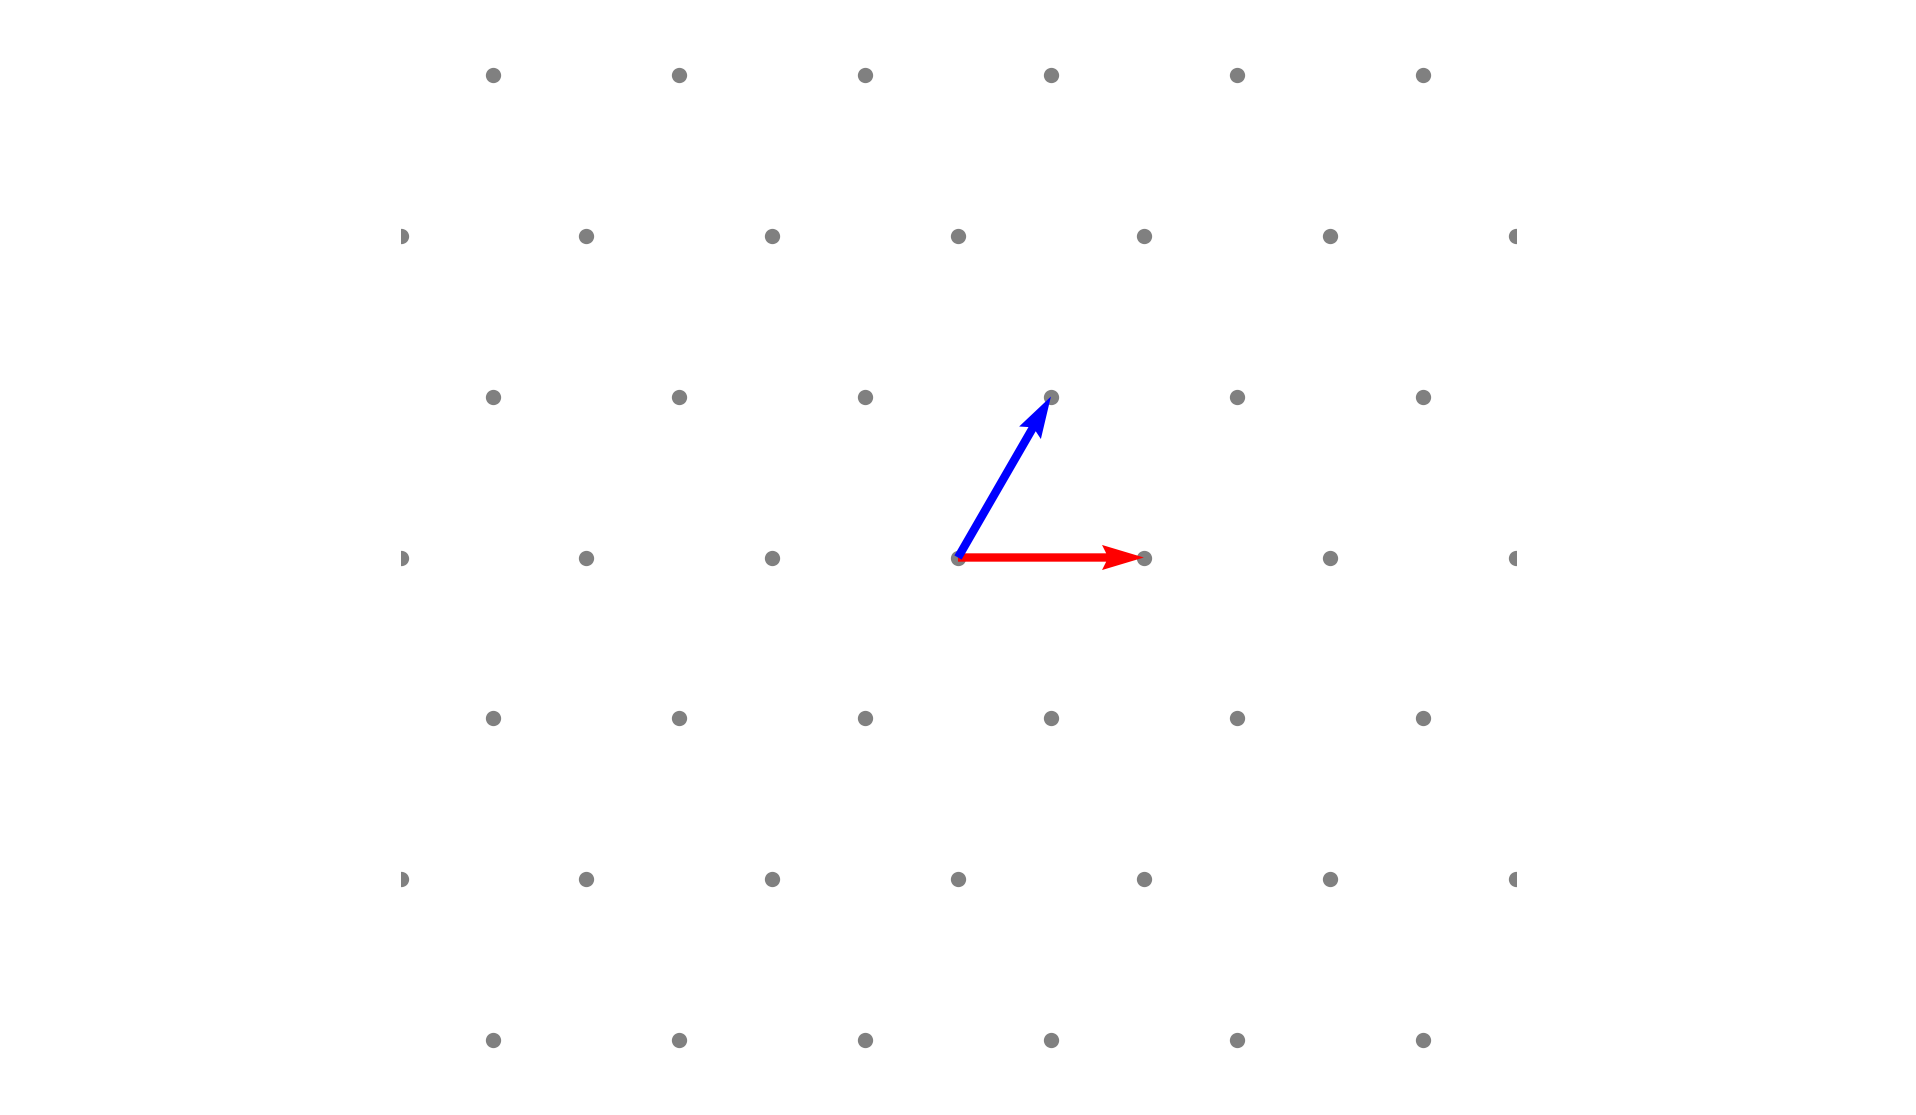
\includegraphics[width=\linewidth]{a2_good_basis.png}
        \end{column}
    \end{columns}
\end{frame}

%------------------------------------------------

\begin{frame}
    \frametitle{What is a lattice?}
    \begin{columns}[T]
        \begin{column}{0.48\linewidth}
            \begin{center}
            \begin{tcolorbox}[colback=ICLBlue!5!white,colframe=ICLBlue,title=\textbf{Definition:} Lattice]
                The set of all linear integer combinations of basis vectors,
                \[
                    \mathcal{L} = \{ \sum_{i = 1}^{d}\mathbf{b}_i\mathbf{x} \ | \ \mathbf{x} \in \mathbb{Z}^d \}
                \]
            \end{tcolorbox}

            \[
                \mathbf{B'} = \begin{pmatrix}
                    \color{red}\frac{5}{2} & \color{blue}2\\
                    \color{red}\frac{\sqrt{3}}{2} & \color{blue}\sqrt{3}
                \end{pmatrix}
            \]
            \end{center}
        \end{column}
        \begin{column}{0.48\linewidth}
            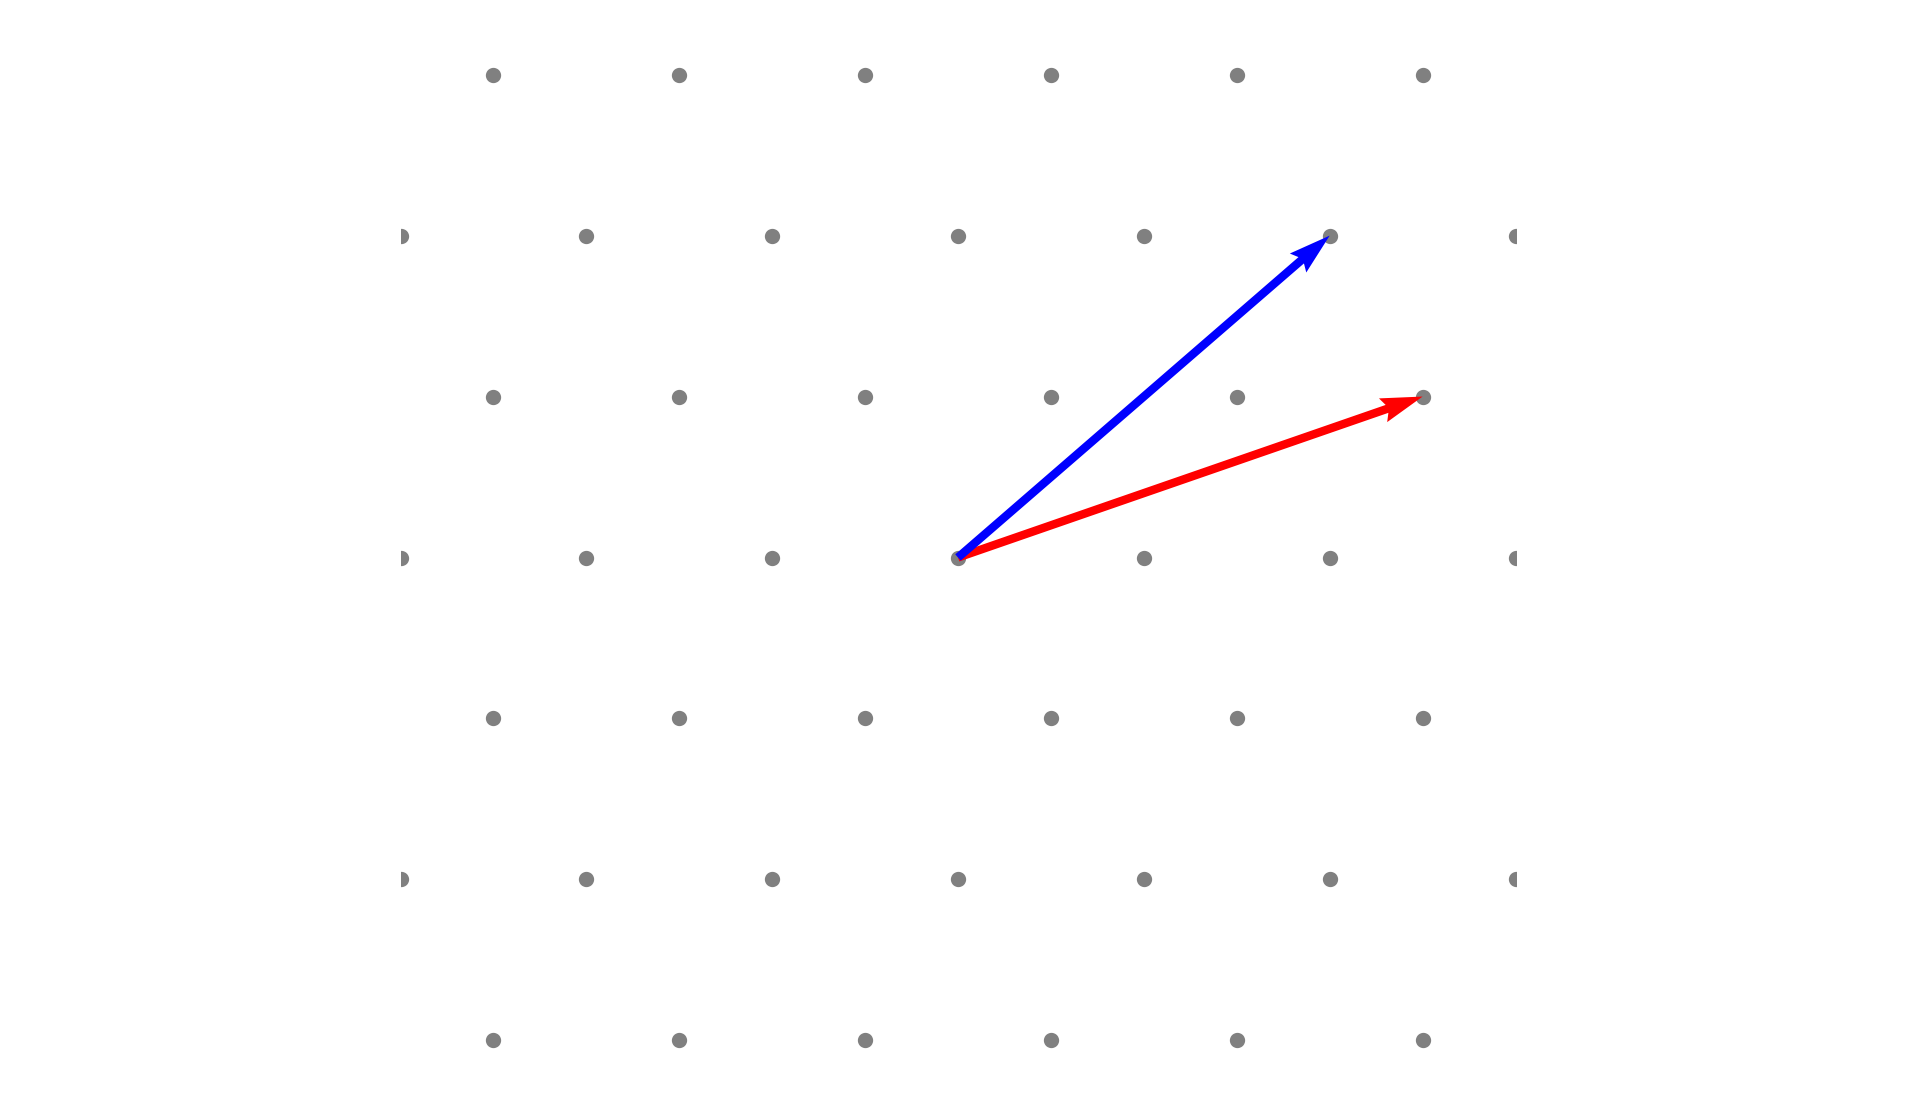
\includegraphics[width=\linewidth]{a2_bad_basis.png}
        \end{column}
    \end{columns}
\end{frame}

%------------------------------------------------

\begin{frame}
    \frametitle{What is a lattice?}
    \begin{columns}[T]
        \begin{column}{0.33\linewidth}
            \begin{center}
                \begin{tcolorbox}[colback=ICLBlue!5!white,colframe=ICLBlue,title=\textbf{Good Basis}]
            \begin{itemize}
                \item Short vectors
                \item Orthogonal
            \end{itemize}
            \end{tcolorbox}
            \end{center}
        \end{column}
        \begin{column}{0.33\linewidth}
            \begin{center}
                \Huge
                \(\color{green}\longrightarrow\)\\
                \vspace{20pt}
                \(\color{red}\longleftarrow\)
                \normalsize
            \end{center}
        \end{column}
        \begin{column}{0.33\linewidth}
            \begin{center}
                \begin{tcolorbox}[colback=ICLBlue!5!white,colframe=ICLBlue,title=\textbf{Bad Basis}]
            \begin{itemize}
                \item Long vectors
                \item Not orthogonal
            \end{itemize}
            \end{tcolorbox}
            \end{center}
        \end{column}
    \end{columns}
    This process of going from a bad to good basis is called \textbf{basis reduction}.
    \begin{columns}
        \begin{column}{0.33\linewidth}
                \begin{tcolorbox}[colback=ICLBlue!5!white,colframe=ICLBlue,title=\textbf{LLL}]
                    \begin{itemize}
                        \item Polynomial runtime (in dimension)
                        \item Exponential approximation (in dimension)
                    \end{itemize}
                \end{tcolorbox}
        \end{column}
        \begin{column}{0.33\linewidth}
                \begin{tcolorbox}[colback=ICLBlue!5!white,colframe=ICLBlue,title=\textbf{BKZ}]
                    \begin{itemize}
                        \item Exponential runtime (in blocksize)
                        \item Exponential approximation (in blocksize)
                    \end{itemize}
                \end{tcolorbox}
        \end{column}
        \begin{column}{0.33\linewidth}
                \begin{tcolorbox}[colback=ICLBlue!5!white,colframe=ICLBlue,title=\textbf{HKZ}]
                    \begin{itemize}
                        \item Exponential runtime (in dimension)
                        \item Optimal output
                    \end{itemize}
                \end{tcolorbox}
        \end{column}
    \end{columns}
\end{frame}

%------------------------------------------------

\begin{frame}
    \frametitle{What are hard lattice problems?}

    \begin{adjustwidth}{0cm}{0cm} % The first parameter is the left margin indentation and the second is the right margin indentation

        \begin{tcolorbox}[colback=ICLBlue!5!white,colframe=ICLBlue,title=\textbf{Definition:} Shortest Vector Problem (SVP)]
            Given a lattice, find the shortest \textit{non-zero} lattice point.
        \end{tcolorbox}

        \begin{tcolorbox}[colback=ICLBlue!5!white,colframe=ICLBlue,title=\textbf{Definition:} Learning With Errors Problem (LWE)]
            Let, $\color{ForestGreen} \begin{bmatrix} \\ \mathbf{b} \\ \\ \end{bmatrix} \color{black} = \color{ForestGreen} \begin{bmatrix} & & \\ & \mathbf{A} & \\ & & \end{bmatrix} \color{black} \begin{bmatrix} \\ \mathbf{s} \\ \\ \end{bmatrix} + \begin{bmatrix} \\ \mathbf{e} \\ \\ \end{bmatrix}$.
            Knowing \textit{only} the values in \color{ForestGreen} green\color{black}, find $\begin{bmatrix} \\ \mathbf{s} \\ \\ \end{bmatrix}$.
        \end{tcolorbox}
        \begin{tcolorbox}[colback=ICLBlue!5!white,colframe=ICLBlue,title=\textbf{Definition:} Lattice Isomorphism Problem (LIP)]
            Given two lattices, $\mathcal{L}_1$ and $\mathcal{L}_2$, find the scaling factor and rotation to send one to the other (if it exists).
        \end{tcolorbox}

        But we also have the Short Integer Solutions problem (SIS), the NTRU problem, the Closest Vector Problem (CVP), and all the many variants of anything mentioned here!

    \end{adjustwidth}
\end{frame}

%------------------------------------------------

\begin{frame}
    \frametitle{Closest Vector Problem}
        \begin{tcolorbox}[colback=ICLBlue!5!white,colframe=ICLBlue,title=\textbf{Definition:} Closest Vector Problem (CVP)]
            Given a lattice and a random point, find the closest lattice point.
        \end{tcolorbox}

        \begin{columns}[T]
            \begin{column}{0.48\linewidth}
                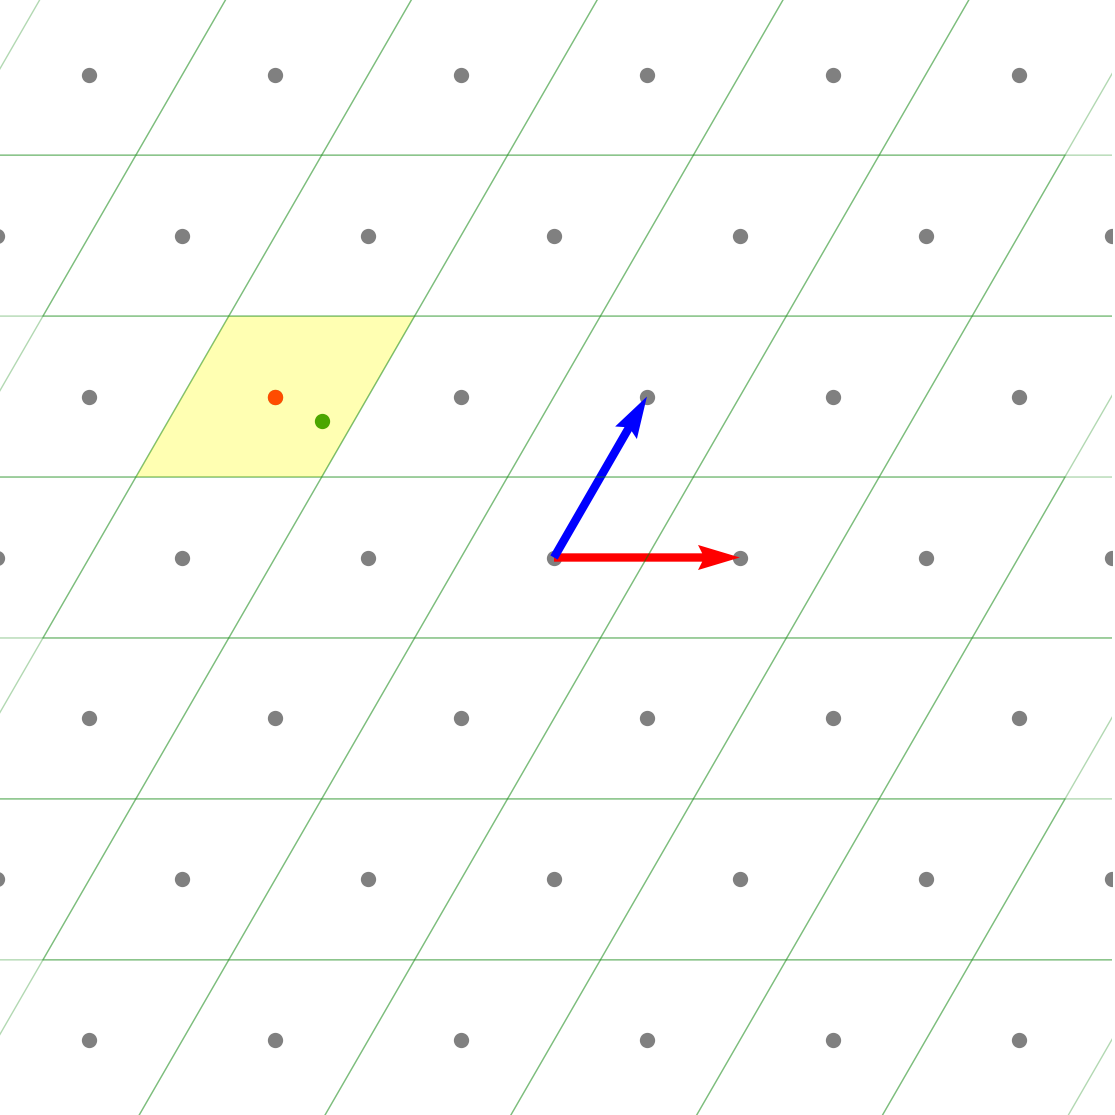
\includegraphics[width=\linewidth]{cvp_good_basis.png}
            \end{column}
            \begin{column}{0.48\linewidth}
                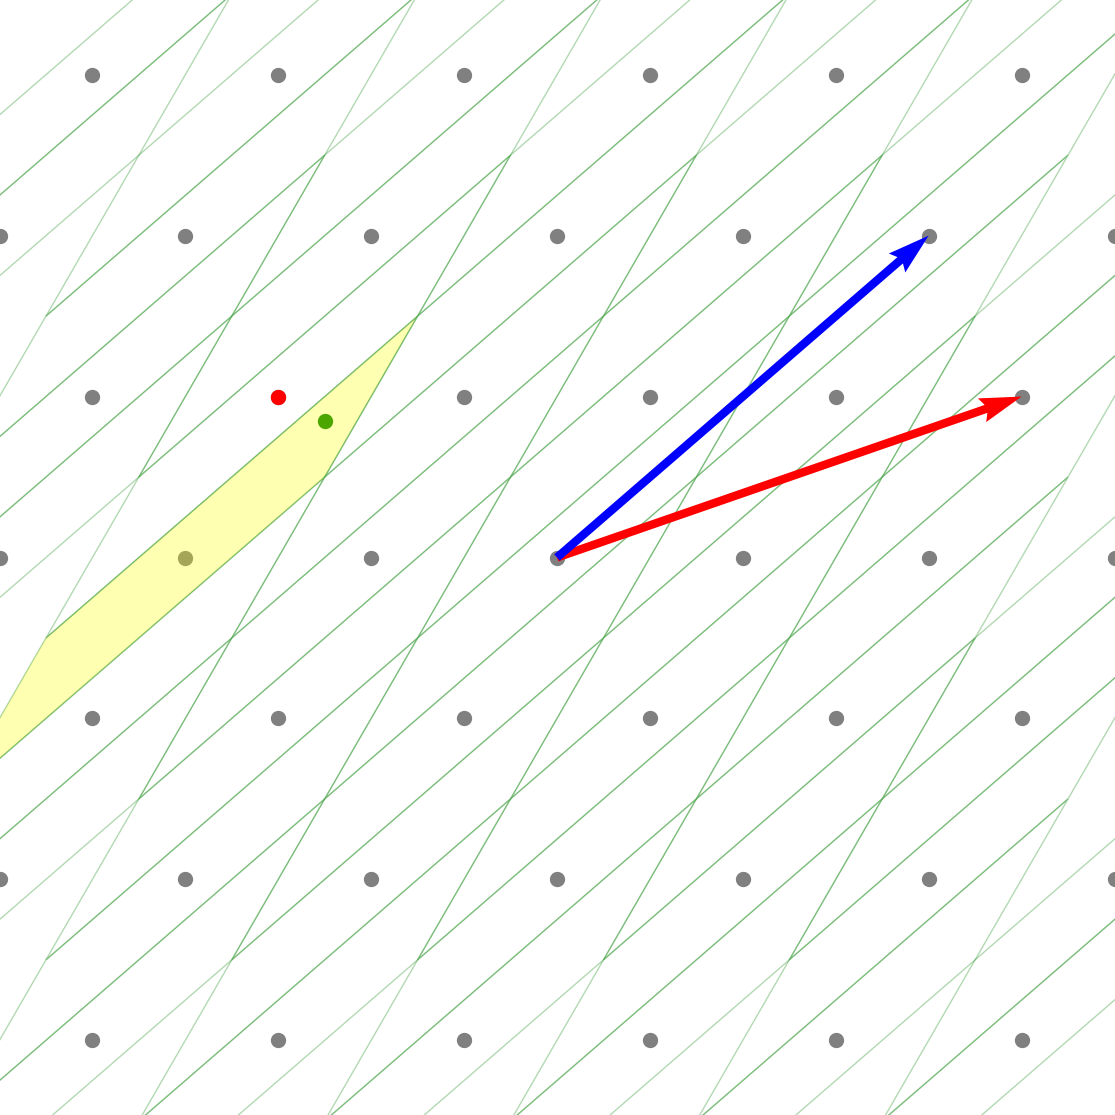
\includegraphics[width=\linewidth]{cvp_bad_basis.png}
            \end{column}
        \end{columns}
\end{frame}

%------------------------------------------------

\begin{frame}
    \frametitle{Learning With Errors}
    \begin{columns}[T] % [T] ensures correct vertical alignment
        \begin{column}{0.48\linewidth} % Left column
            \begin{tcolorbox}[colback=ICLBlue!5!white,colframe=ICLBlue,title=Learning With Errors Problem (LWE)]
                \[
                    \color{ForestGreen} \begin{bmatrix} \\ \mathbf{b} \\ \\ \end{bmatrix} \color{black} = \color{ForestGreen} \begin{bmatrix} & & \\ & \mathbf{A} & \\ & & \end{bmatrix} \color{red} \begin{bmatrix} \\  \mathbf{s} \\ \\ \end{bmatrix} \color{black} + \begin{bmatrix} \\ \mathbf{e} \\ \\ \end{bmatrix}
                \]
            \end{tcolorbox}

            We can construct what is called a $q$-ary lattice using $\mathbf{A}$.

            Then, taking the target vector $\mathbf{b}$, solving a CVP instance \textit{should} give us $\mathbf{As}$, and therefore $\mathbf{s}$.

            Unfortunately, if the LWE parameters are chosen well, we do not get a good basis for our new lattice, and so solving CVP is hard.
        \end{column}
        \begin{column}{0.48\linewidth} % Right column
            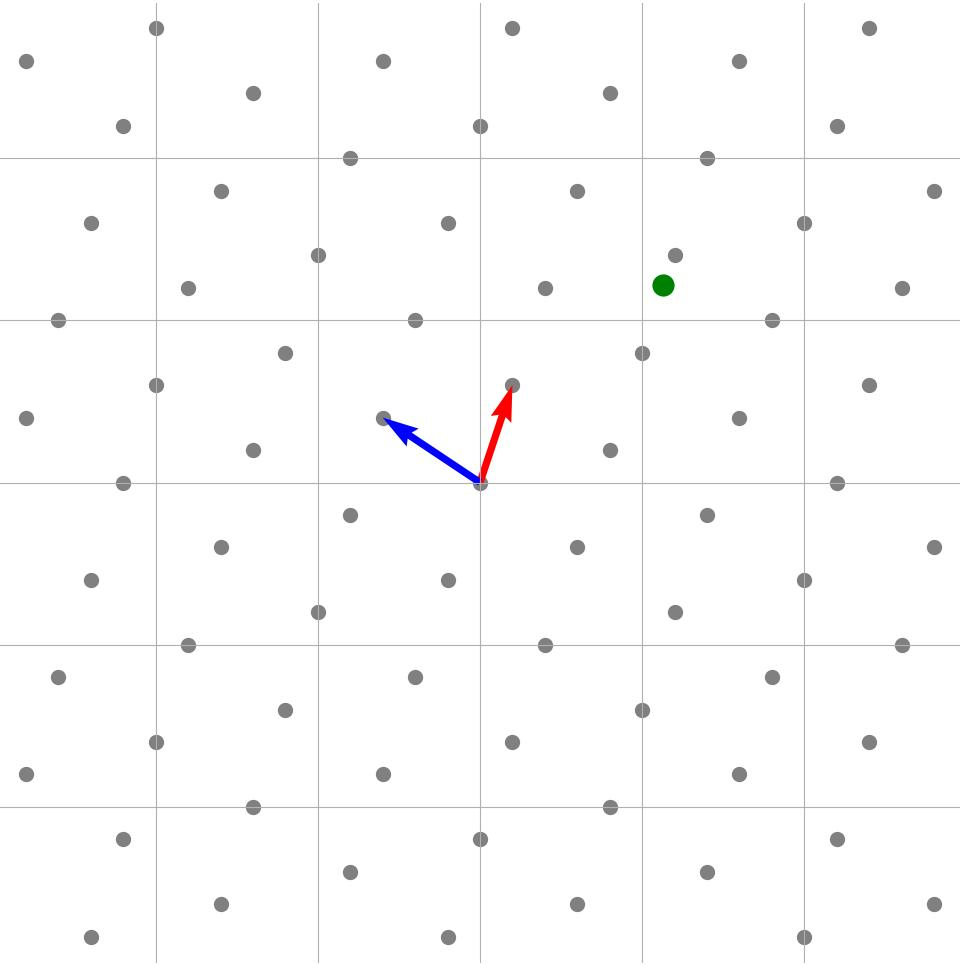
\includegraphics[width=\linewidth]{lwe_lattice.jpeg} % Trimming is used to crop your image and the order of dimensions is: left, bottom, right, top. It's recommended to crop outside of LaTeX though, to ensure the aspect ratio remains the same.
        \end{column}
    \end{columns}
\end{frame}

%------------------------------------------------

\begin{frame}
    \frametitle{Learning With Errors}
    \begin{columns}[T] % [T] ensures correct vertical alignment
        \begin{column}{0.48\linewidth} % Left column
            \begin{tcolorbox}[colback=ICLBlue!5!white,colframe=ICLBlue,title=Learning With Errors Problem (LWE)]
                \[
                    \color{ForestGreen} \begin{bmatrix} \\ \mathbf{b} \\ \\ \end{bmatrix} \color{black} = \color{ForestGreen} \begin{bmatrix} & & \\ & \mathbf{A} & \\ & & \end{bmatrix} \color{red} \begin{bmatrix} \\  \mathbf{s} \\ \\ \end{bmatrix} \color{black} + \begin{bmatrix} \\ \mathbf{e} \\ \\ \end{bmatrix}
                \]
            \end{tcolorbox}

            With a good basis for our lattice, something that can be kept secret, solving CVP and recovering the secret is easy, however.

            One of the key parts of proving the security of LWE is that the vector \(\mathbf{b}\) is indistinguishable from a random vector.
        \end{column}
        \begin{column}{0.48\linewidth} % Right column
            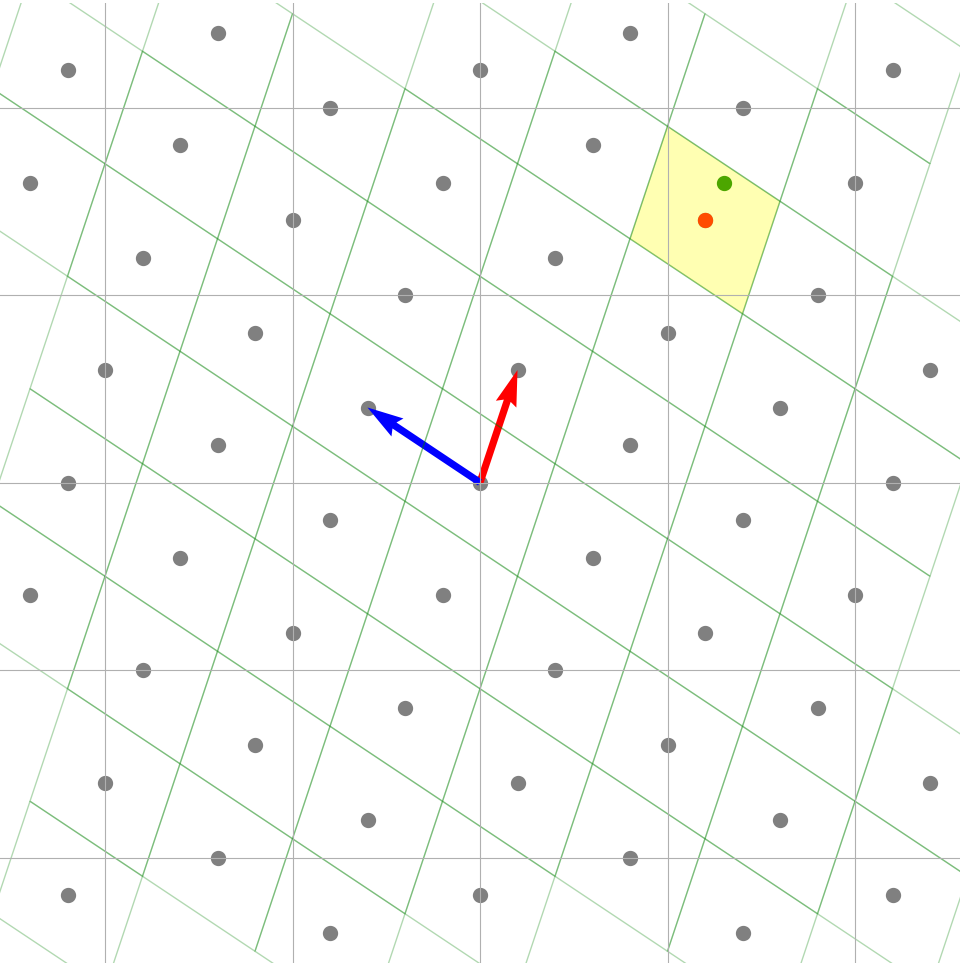
\includegraphics[width=\linewidth]{lwe_lattice_solved.png} % Trimming is used to crop your image and the order of dimensions is: left, bottom, right, top. It's recommended to crop outside of LaTeX though, to ensure the aspect ratio remains the same.
        \end{column}
    \end{columns}
\end{frame}

%------------------------------------------------

\begin{frame}
    \frametitle{Lattice Isomorphism Problem}
    \begin{columns}[T] % [T] ensures correct vertical alignment
        \begin{column}{0.48\linewidth} % Left column
            \includegraphics[height=70mm]{lip_in_the_wild.jpeg} % Trimming is used to crop your image and the order of dimensions is: left, bottom, right, top. It's recommended to crop outside of LaTeX though, to ensure the aspect ratio remains the same.
        \end{column}
        \begin{column}{0.48\linewidth}
            \begin{tcolorbox}[colback=ICLBlue!5!white,colframe=ICLBlue,title=Lattice Isomorphism Problem (LIP)]
                Given two lattices $\mathcal{L}_1$ and $\mathcal{L}_2$, find the \textit{isometry} between the two lattices.

                In other words, find the translation that describes the rotation that sends $\mathcal{L}_1$ to $\mathcal{L}_2$.
            \end{tcolorbox}
            This is the $A_2$ lattice, the densest sphere packing in two dimensions.

            Here, the rotation is $90^\circ$, with a scaling factor of $1$.
        \end{column}
    \end{columns}
\end{frame}

%------------------------------------------------

\begin{frame}
    \frametitle{Lattice Isomorphism Problem}
    \begin{columns}[T]
        \begin{column}{0.48\linewidth}
            First, we take a lattice that has nice properties (dense, good decoding etc.).

        \end{column}
        \begin{column}{0.48\linewidth}
            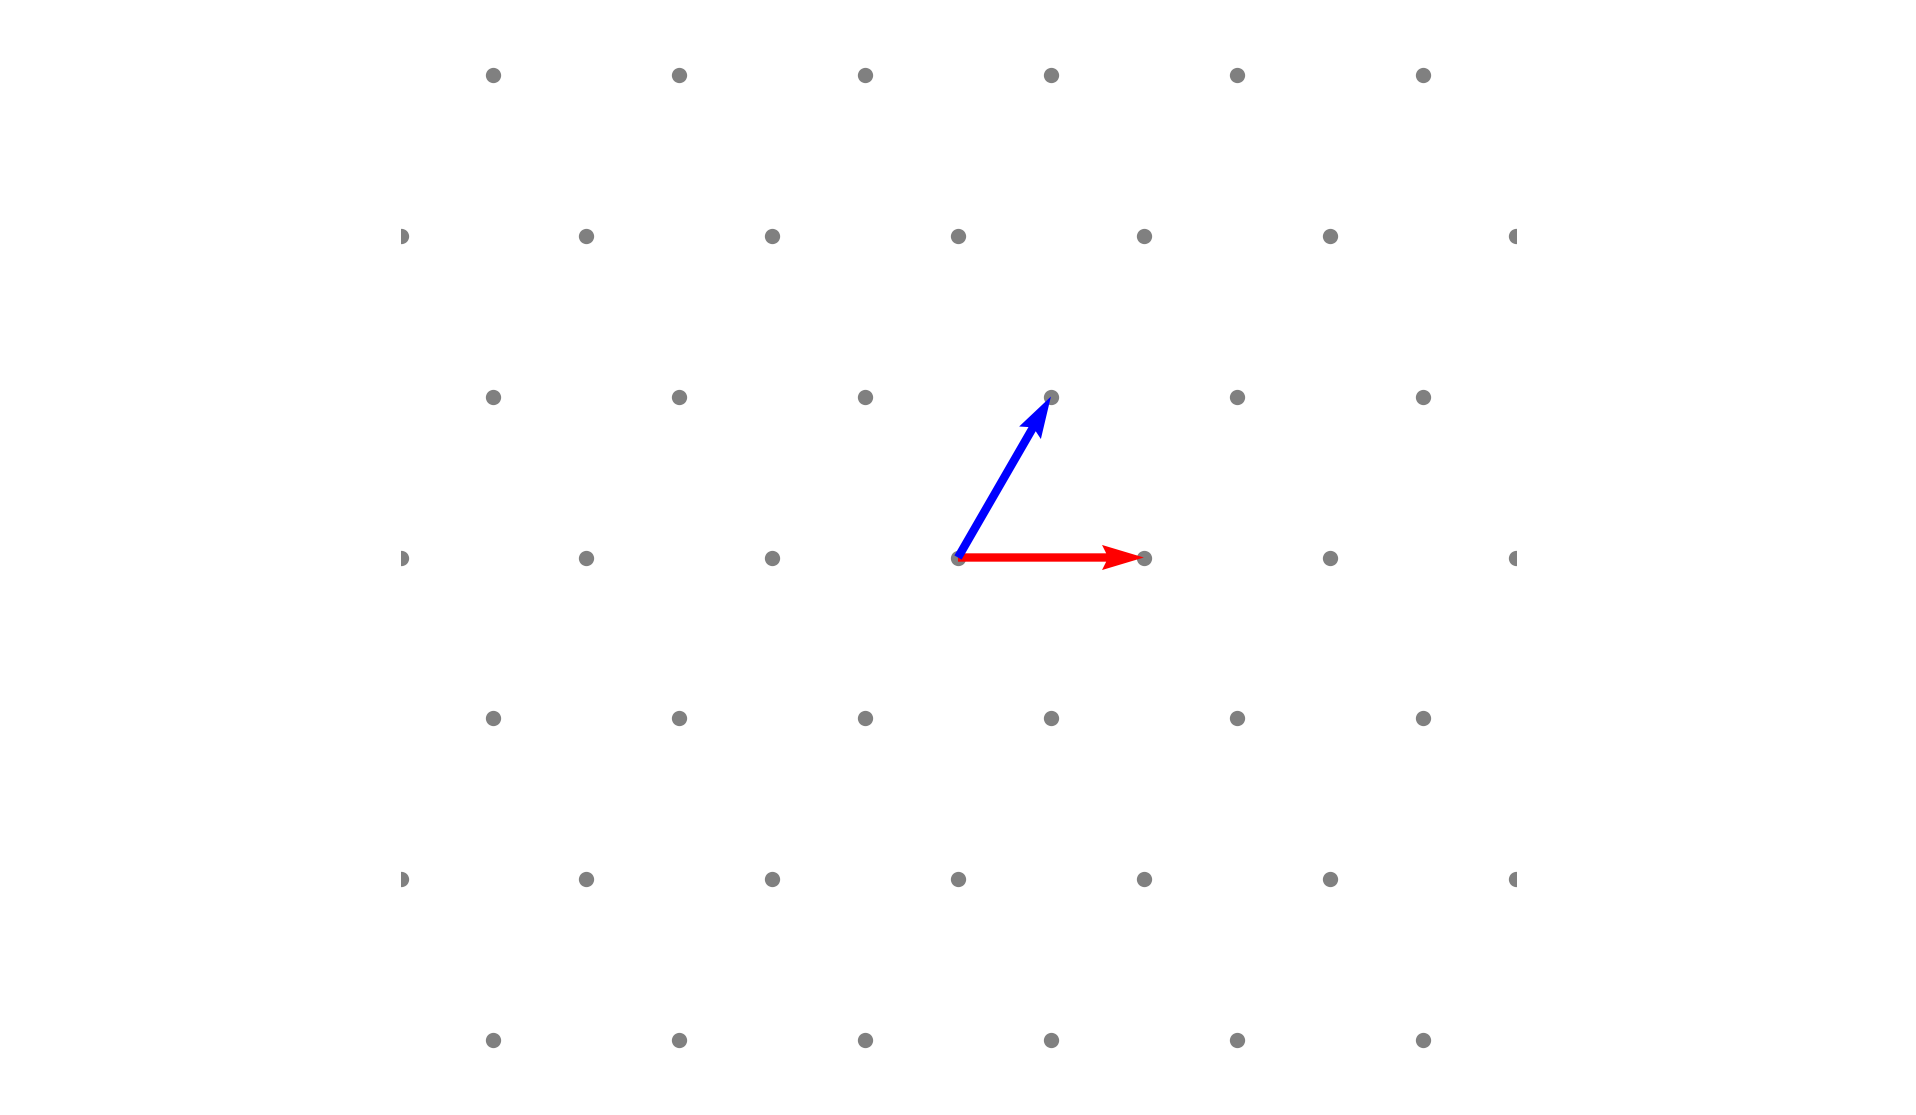
\includegraphics[width=\linewidth]{a2_good_basis.png}
        \end{column}
    \end{columns}
\end{frame}

%------------------------------------------------

\begin{frame}
    \frametitle{Lattice Isomorphism Problem}
    \begin{columns}[T]
        \begin{column}{0.48\linewidth}
            First, we take a lattice that has nice properties (dense, good decoding etc.).

            Then, we apply some \textbf{unimodular} transform. This equates to a rotation of our original lattice, and we say that these two are \textbf{isomorphic}.

        \end{column}
        \begin{column}{0.48\linewidth}
            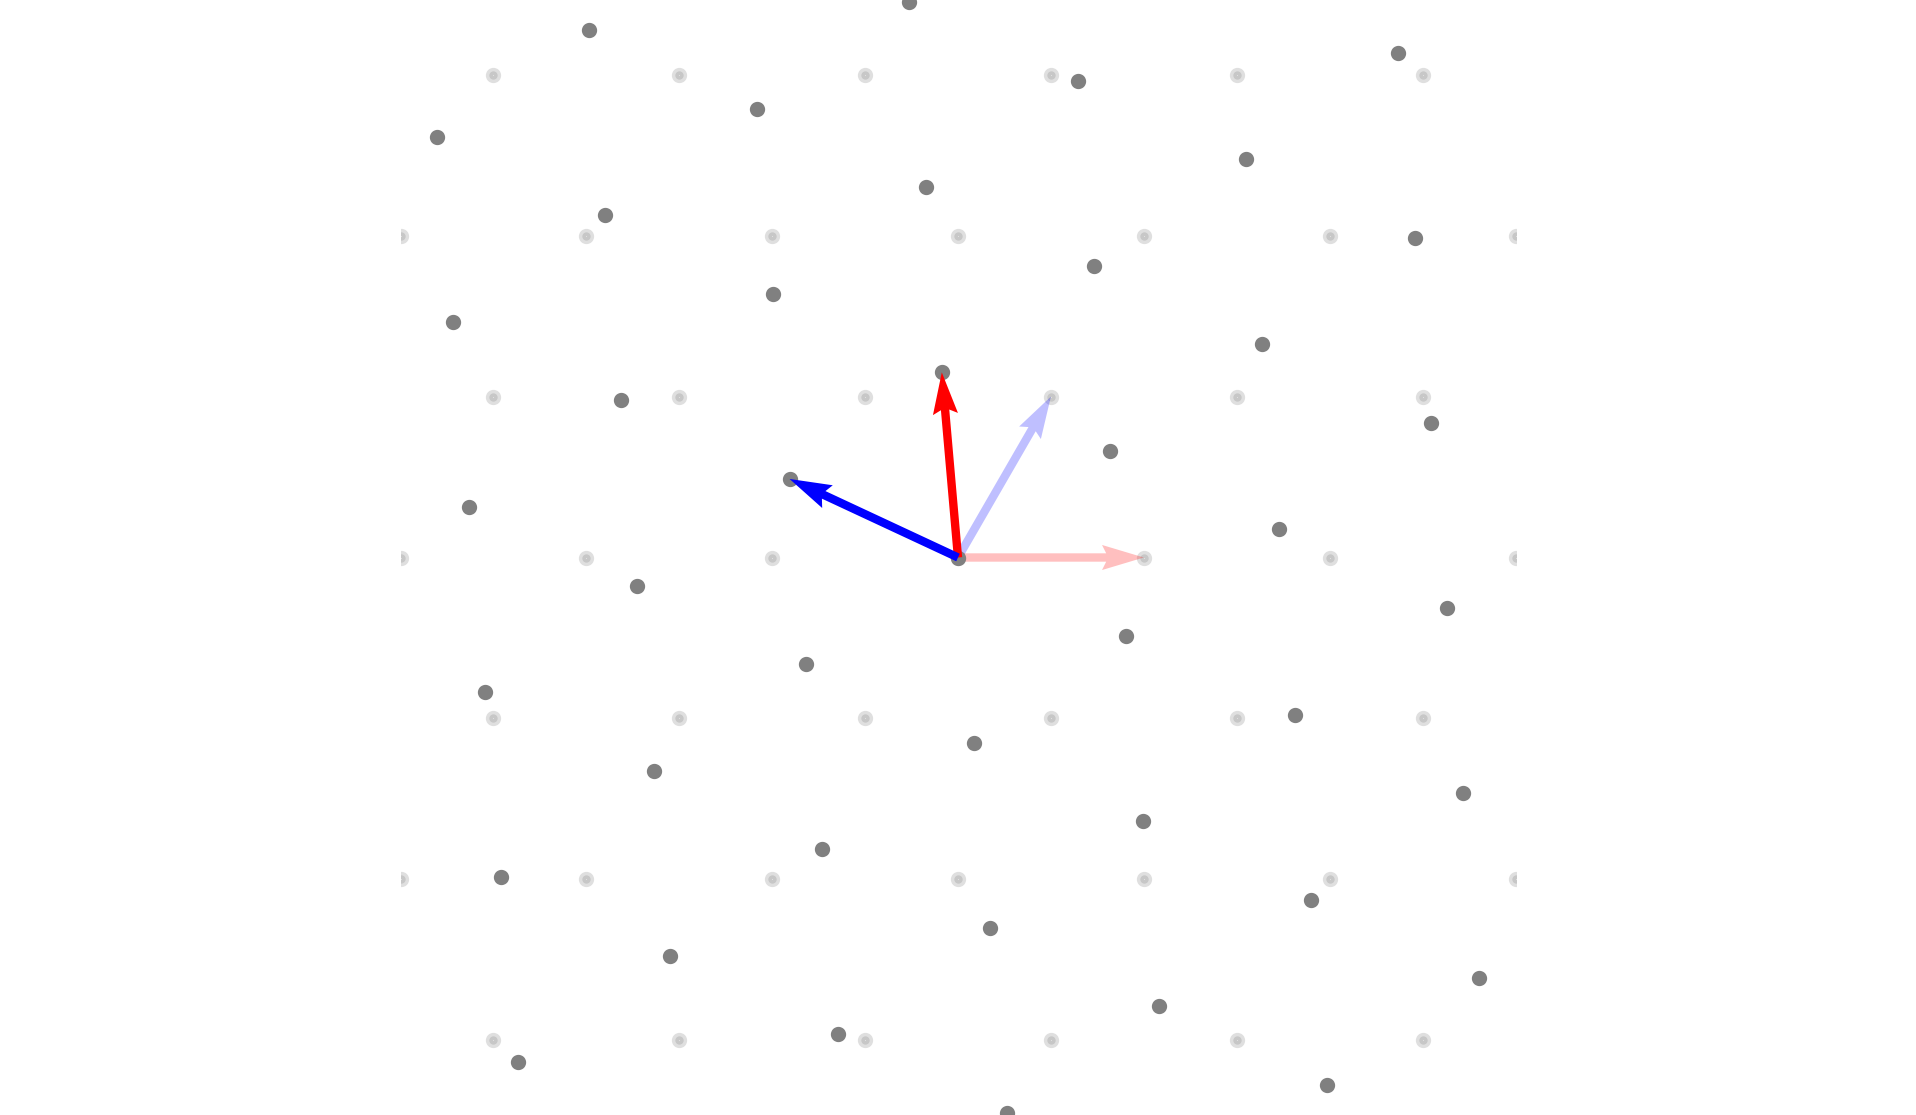
\includegraphics[width=\linewidth]{a2_rotated_basis.png}
        \end{column}
    \end{columns}
\end{frame}

%------------------------------------------------

\begin{frame}
    \frametitle{Lattice Isomorphism Problem}
    \begin{columns}[T]
        \begin{column}{0.48\linewidth}
            First, we take a lattice that has nice properties (dense, good decoding etc.).

            Then, we apply some \textbf{unimodular} transform. This equates to a rotation of our original lattice, and we say that these two are \textbf{isomorphic}.

            Finally, we hide this rotation with a basis transform; we make a bad basis of this isomorphism.
        \end{column}
        \begin{column}{0.48\linewidth}
            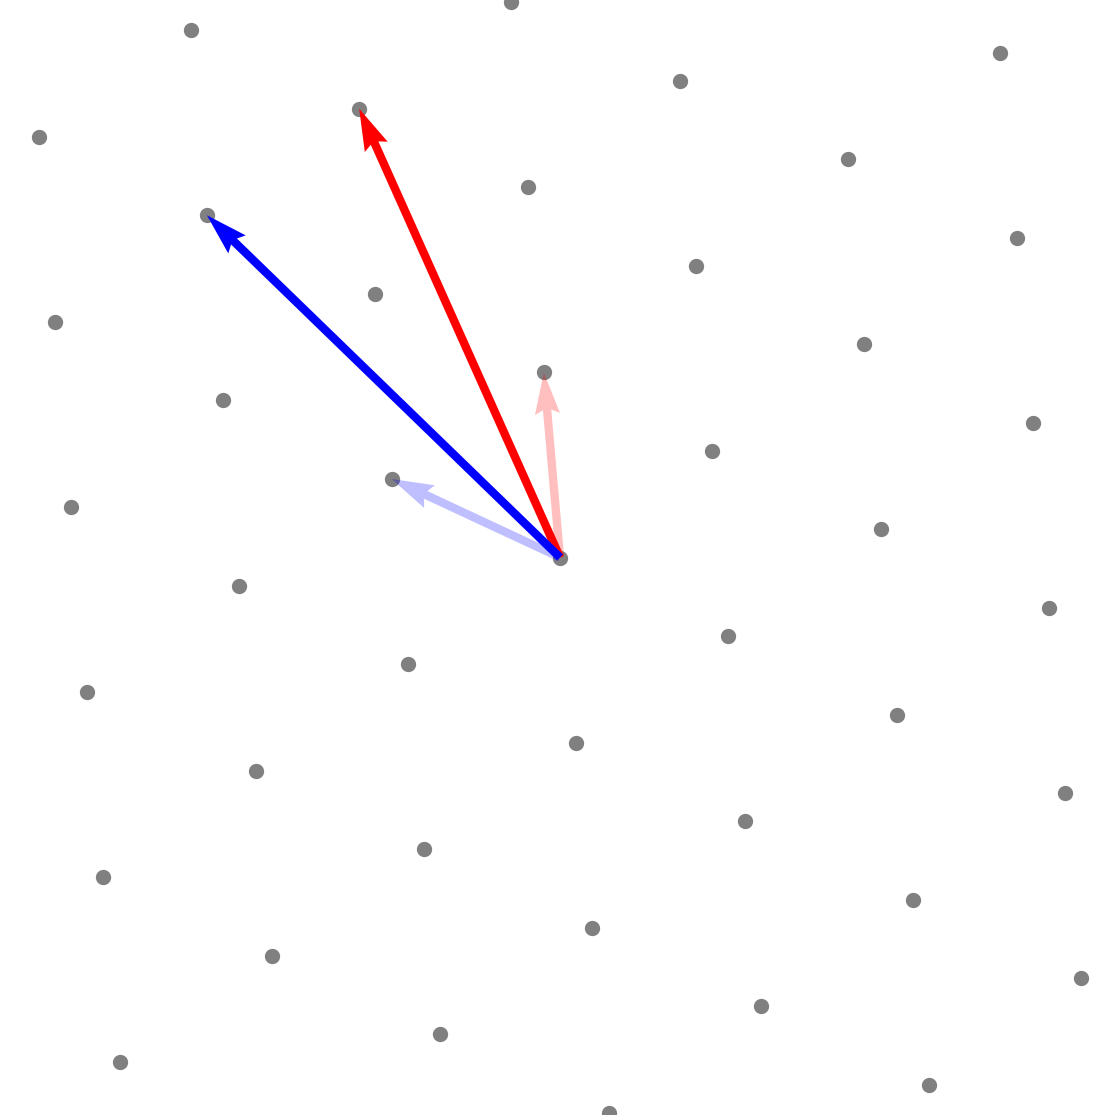
\includegraphics[width=\linewidth]{a2_rotated_basis_change.png}
        \end{column}
    \end{columns}
\end{frame}

%------------------------------------------------

\begin{frame}
    \frametitle{Lattice Isomorphism Problem}
    \begin{columns}[T]
        \begin{column}{0.48\linewidth}
            To encrypt, we take our message, a lattice point in the public lattice and add some small error.
            
            Recovering this original lattice point using the (bad) public basis is hard to do.
        \end{column}
        \begin{column}{0.48\linewidth}
            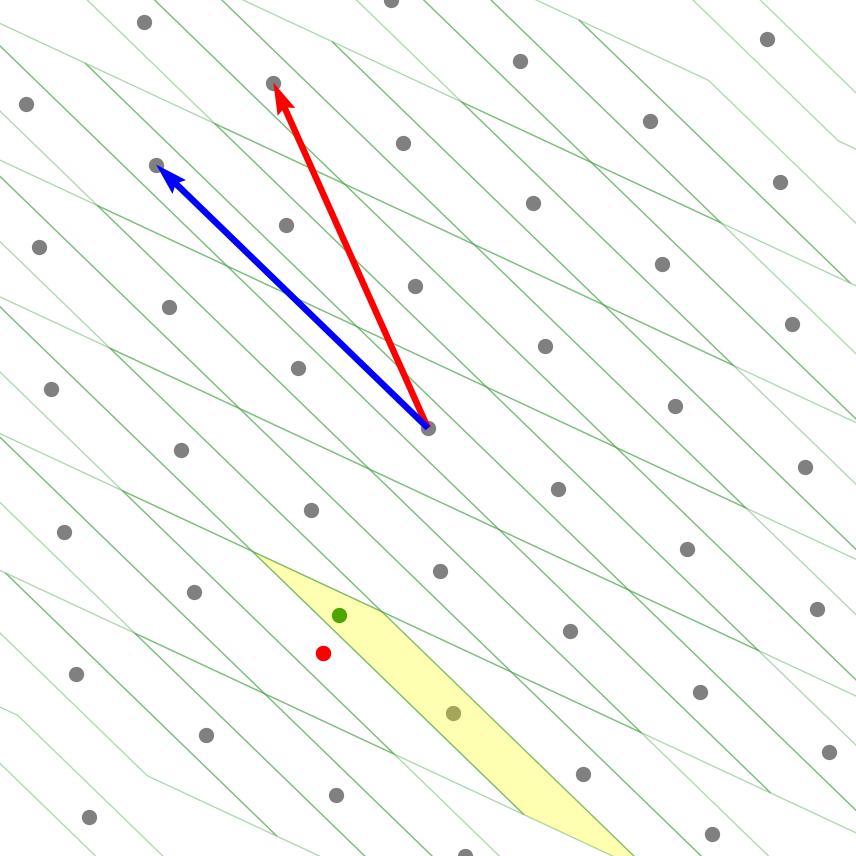
\includegraphics[width=\linewidth]{LIP_bad_basis.png}
        \end{column}
    \end{columns}
\end{frame}

%------------------------------------------------

\begin{frame}
    \frametitle{Lattice Isomorphism Problem}
    \begin{columns}[T]
        \begin{column}{0.48\linewidth}
            To encrypt, we take our message, a lattice point in the public lattice and add some small error.
            
            Recovering this original lattice point using the (bad) public basis is hard to do.

            Knowing the rotation, we can convert this back to our original lattice, which we know a good basis for, and can easily recover the corresponding lattice point.
        \end{column}
        \begin{column}{0.48\linewidth}
            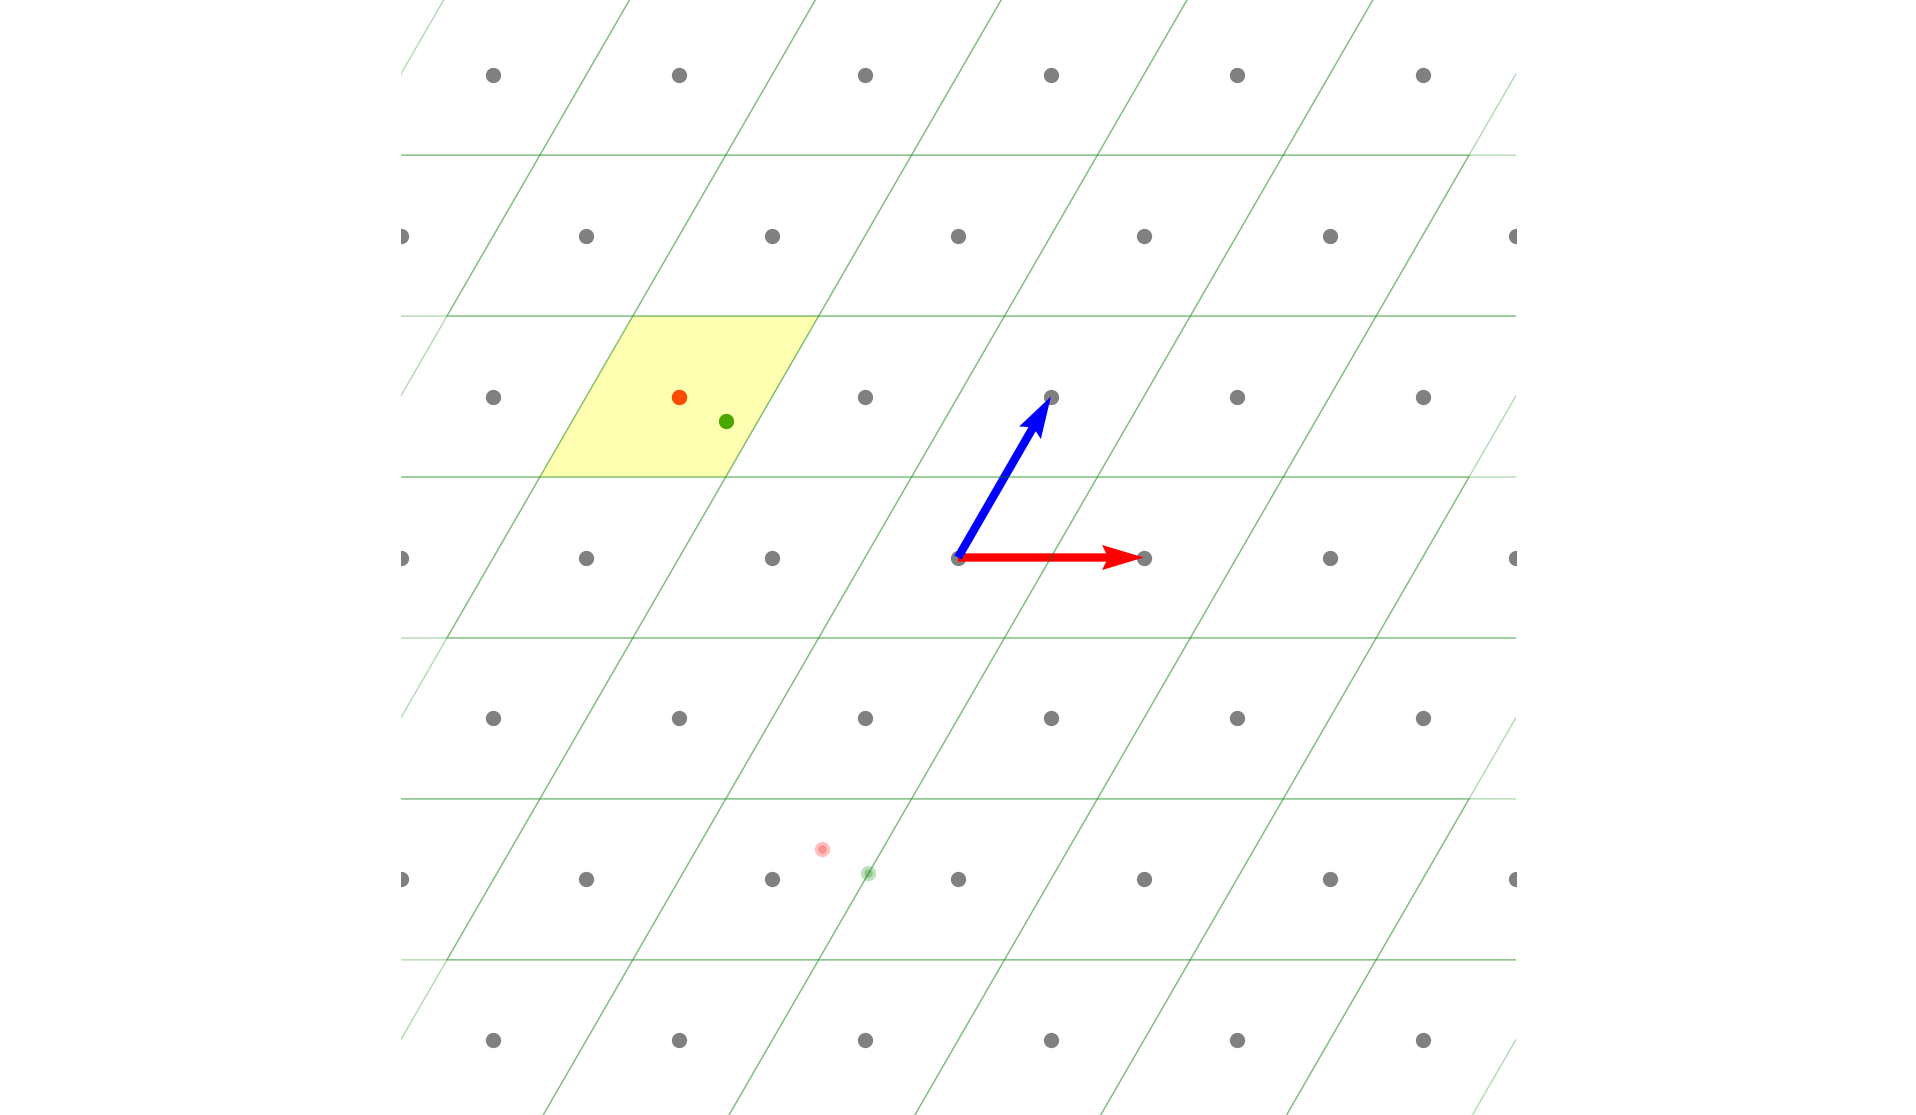
\includegraphics[width=\linewidth]{LIP_good_basis.png}
        \end{column}
    \end{columns}
\end{frame}

%------------------------------------------------

\begin{frame}
    \frametitle{It's all SVP?}

    \begin{columns}[T] % [T] ensures correct vertical alignment
        \begin{column}{0.58\linewidth} % Left column
            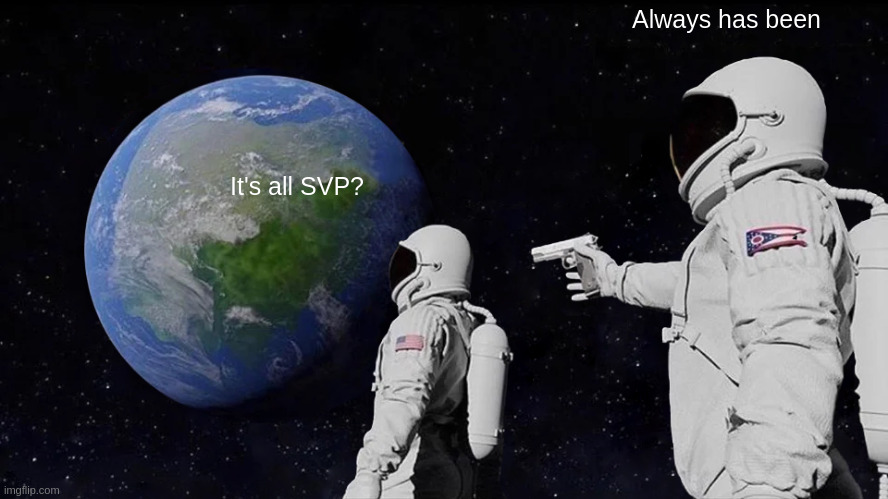
\includegraphics[width=0.9\linewidth]{always_has_been.jpg} % Trimming is used to crop your image and the order of dimensions is: left, bottom, right, top. It's recommended to crop outside of LaTeX though, to ensure the aspect ratio remains the same.

            \vspace{-1.5em}{\tiny\textcolor{ICLBlue}{(Above) Regev discovering the the LWE to $\gamma$-SVP reduction, 2005}}\newline

            \vspace{-2em}All of the above problems are reducible to (approximate)-SVP. It can easily be seen that solving CVP solves them, but to solve CVP you need a good basis.
            To get a good basis, you need to find short vectors - i.e. solve SVP.
        \end{column}
        \begin{column}{0.38\linewidth} % Right column
            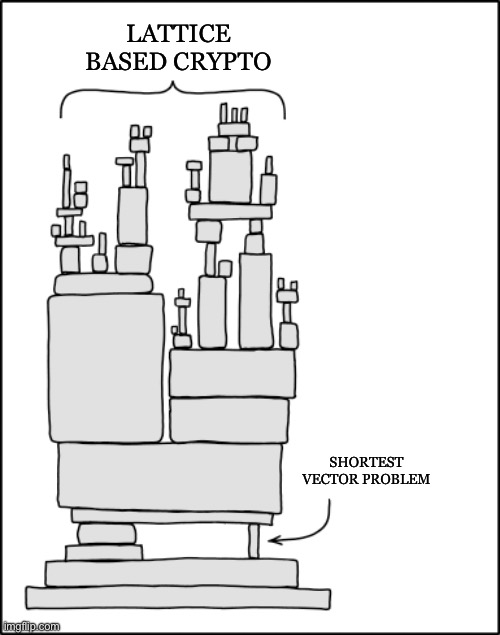
\includegraphics[width=0.85\linewidth]{svp_crutch.jpeg} % Trimming is used to crop your image and the order of dimensions is: left, bottom, right, top. It's recommended to crop outside of LaTeX though, to ensure the aspect ratio remains the same.

            \vspace{-1.5em}{\tiny\textcolor{ICLBlue}{(Above) xkcd Dependency, lattice based cryptography special edition}}
        \end{column}
    \end{columns}
\end{frame}

%------------------------------------------------

\begin{frame}
    \frametitle{The PQC timeline}
    \begin{columns}
        \begin{column}{0.5\linewidth} % Right column
            \begin{itemize}
                \item \textbf{Deprecated}: \\the algorithm and key length/strength may be used, but there is some security risk. Assess risk before using a deprecated algorithm or key length.
            \end{itemize}
        \end{column}
        \begin{column}{0.5\linewidth} % Right column
            \begin{itemize}
                \item \textbf{Disallowed}: \\the algorithm, key length/strength, parameter set, or scheme is no longer allowed for the stated purpose.
            \end{itemize}
        \end{column}
    \end{columns}
    \begin{columns}
        \begin{column}{0.58\linewidth} % Left column
        \vspace{-2em}
            \begin{table}[]
                \begin{tabular}{|l|l|l|}
                    \hline
                    \textbf{Scheme} & \textbf{Deprecated} & \textbf{Disallowed} \\
                                    & \textit{(112 bit strength only)}& \\
                    \hline
                    \textit{Key Establishment}&&\\
                    Finite Field DH and MQV & 2030 & 2035 \\
                    Elliptic Curve DH and MQV & 2030 & 2035 \\
                    RSA & 2030 & 2035 \\
                    \hline
                    \textit{Signatures}&&\\
                    ECDSA & 2030 & 2035 \\
                    EdDSA & - & 2035 \\
                    RSA & 2030 & 2035 \\
                    \hline
                \end{tabular}
            \end{table}
        \end{column}
        \begin{column}{0.32\linewidth} % Left column
            \newline
            \textbf{Replace with:}\\
            \textit{Key Establishment}
            \vspace{-1em}
            \begin{itemize}
                \item ML-KEM
            \end{itemize}
            \textit{Signatures}
            \vspace{-1em}
            \begin{itemize}
                \item ML-DSA
                \item SLH-DSA
                \item LMS, HSS
                \item XMSS
            \end{itemize}
        \end{column}
    \end{columns}
\end{frame}

%------------------------------------------------

\begin{frame}
    \frametitle{What does all this mean for me?}
    \begin{adjustwidth}{0cm}{0.15\textwidth} % The first parameter is the left margin indentation and the second is the right margin indentation
        \begin{itemize}
            \item You should begin to use hybrid encryption now
            \begin{itemize}
                \item Especially if a ``harvest now, decrypt later'' threat is relevant to you
                \item Have the fallback of ECC if PQC is broken
                \item Schemes such as X-wing and Xyber768
            \end{itemize}
            \item For most people, this is as simple as upgrading your browser and dependencies (most crypto is dependent on upstream libs like openSSL)
        \end{itemize}
        \vspace{1.5em}
        \begin{quote}
            ``Any digital system that uses existing public standards for public‑key cryptography, or that is planning to transition to such cryptography, could be vulnerable to an attack by a Cryptographically Relevant Quantum Computer (CRQC). To mitigate this risk, the United States must prioritize the timely and equitable transition of cryptographic systems to quantum-resistant cryptography, with the goal of mitigating as much of the quantum risk as is feasible by 2035.''\footfullcite{nsm10}
        \end{quote}
    \end{adjustwidth}
\end{frame}

%------------------------------------------------

\begin{frame}
    \frametitle{Further reading}
    \begin{columns}[T] % [T] ensures correct vertical alignment
        \begin{column}{0.25\linewidth} % Right column
            \centering{\textbf{General\\Cryptography:}}
            
\includegraphics[width=\linewidth]{general.png}
        \end{column}
        \begin{column}{0.25\linewidth} % Left column
            \centering{\textbf{Lattices and\\Lattice Cryptography:}}
            
\includegraphics[width=\linewidth]{lattices_resources.png}
        \end{column}
        \begin{column}{0.25\linewidth} % Center column
            \centering{\textbf{PQC\\Implementations:}}
            
\includegraphics[width=\linewidth]{implementation.png}
        \end{column}
        \begin{column}{0.25\linewidth} % Right column
            \centering{\textbf{Policy, Migration,\\and Standardisation:}}
            
\includegraphics[width=\linewidth]{policy.png}
        \end{column}
    \end{columns}
    
    \begin{center}
        Any other questions please feel free to come talk to me, or email: j.limbrey24@imperial.ac.uk
    \end{center}
\end{frame}
%----------------------------------------------------------------------------------------
%	CLOSING SLIDES
%----------------------------------------------------------------------------------------

% Blue closing slide

\begingroup
	\setbeamercolor{background canvas}{bg=ICLBlue} % Slide background color
	\setbeamercolor{normal text}{fg=white}\usebeamercolor[fg]{normal text} % Slide text color
	\setbeamertemplate{closing slide logo}[logo]{ICL_Logo_White.pdf} % Imperial logo color, use 'ICL_Logo_White.pdf' for white and 'ICL_Logo_Blue.pdf' for blue
	\setbeamertemplate{closing slide text}[text]{Thank you} % Slide text
	
	\usebeamertemplate{closing slide} % Output the closing slide
\endgroup

%----------------------------------------------------------------------------------------

\end{document}
